\section{0426}\label{sec:0426}
\begin{questions}

    \question 对凸多边形
    \begin{parts}
        \part 有多少种三角划分的方法?
        \begin{solution}
            任意一个三角形可以由一条边和不在这条边所在直线上的一个点构成。

            凸多边形的任意一条边都一定属于划分后的一个三角形,任意一个顶点都一定是划分后三角形的一个顶点。
            在凸多边形中,确定一条边后,其他的顶点一定都不在这条边所在的直线上(否则该多边形一定不是凸多边形)。

            \begin{figure}[H]
                \centering
                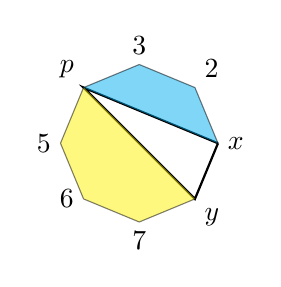
\begin{tikzpicture}
                    \coordinate (p1) at ({0}:1);
                    \coordinate (p2) at ({45}:1);
                    \coordinate (p3) at ({90}:1);
                    \coordinate (p4) at ({135}:1);
                    \coordinate (p5) at ({180}:1);
                    \coordinate (p6) at ({225}:1);
                    \coordinate (p7) at ({270}:1);
                    \coordinate (p8) at ({315}:1);

                    \node[right] at (p1) {$x$};
                    \node[above right] at (p2) {$2$};
                    \node[above] at (p3) {$3$};
                    \node[above left] at (p4) {$p$};
                    \node[left] at (p5) {$5$};
                    \node[left] at (p6) {$6$};
                    \node[below] at (p7) {$7$};
                    \node[below right] at (p8) {$y$};

                    \draw[thick] (p1) -- (p4) -- (p8) -- (p1);
                    \draw[fill=cyan, opacity=0.5] (p1) -- (p2) -- (p3) -- (p4);
                    \draw[fill=yellow, opacity=0.5] (p4) -- (p5) -- (p6) -- (p7) -- (p8);

                \end{tikzpicture}
            \end{figure}

            所以凸$n$边形的一条边可以与其他的$n-2$个点构成三角形,
            且该三角形将原凸多边形分成两个凸多边形,这两个凸多边形可以以相同的算法分划,直到其边数不超过$3$。

            设$T(n)$为一个$n$边形的三角形划分方法。则\[
                T(n) = \begin{cases}
                    0                                & , n = 2 \\
                    1                                & , n = 3 \\
                    \sum_{i = 2}^{n-1}{T(i)T(n-i+1)} & , n > 3
                \end{cases}
            \]
        \end{solution}

        \part 如何使对角线长度之和最小?
        \begin{solution}
            使用与上题相同的归纳方式。

            在$\triangle xpy$是三角形划分后结果中的一个三角形的条件下,
            当多边形对角线长度之和最小时,
            黄色和蓝色两个凸多边形一定达到了使其对角线长度之和分别最小的分划。

            记凸$n$边形为$\left\langle p_1, p_2, \dots , p_n \right\rangle$,
            其对角线长度和最小为$ Q \left( \left\langle p_1, p_2, \dots , p_n \right\rangle \right) $。
            \[
                Q \left( \left\langle p_1, p_2, \dots , p_n \right\rangle \right) =
                \begin{cases}
                    0        & , n \le 3 \\
                    \min_{1 < i < n} \left\{
                    \begin{aligned}
                        Q \left( \left\langle p_1, \dots , p_i \right\rangle \right)
                        + Q \left( \left\langle p_{i}, \dots , p_n \right\rangle \right) \\
                        + D(p_1, p_i) + D(p_n, p_i)
                    \end{aligned}
                    \right\} & , n > 3
                \end{cases}
            \]
            其中,$D(p_i, p_j) = \begin{cases}
                    0               & , |i-j| > 1        \\
                    || p_i - p_j || & , \text{otherwise}
                \end{cases}$

            由于子问题重叠,考虑使用动态规划求解。
            共有$O(n^2)$个子问题需要求解,求解每个子问题所需的时间复杂度为$O(n)$。
            总的时间复杂度为$O(n^3)$

            \textbf{伪代码见算法\ref{alg:0426:1}}
        \end{solution}

        \begin{algorithm}[!ht]
            \caption{最小对角线和}\label{alg:0426:1}
            \begin{algorithmic}[1]
                \Require { $P = \left\langle p_i (x_i, y_i) \right\rangle_{1 \le i \le n}$(要求解的多边形的顶点序列) }
                \Ensure { $S = \left\{ \left\langle p_i, p_j \right\rangle \right\}$(长度和最小的对角线集合) }
                \State $Dist \gets \left\{ \mathsf{Null} \right\}_{n \times n}, Q \gets \left\{ \mathsf{Null} \right\}_{n \times n}$
                \State $(minsum, S) \gets \Call{MinimizeDiagonal}{1,n}$
                \Statex
                \Procedure{Distance}{$i, j$}
                \Comment{获取对角线$p_i - p_j$的长度}
                \If {$Dist[i][j]$ is \textsf{Null}}
                \State $distance \gets \| (x_i,y_i) - (x_j,y_j) \|$ if $|i-j| > 1$ else $0$
                \State $Dist[i][j] \gets distance, Dist[j][i] \gets distance$
                \EndIf
                \State \Return $Dist[i][j]$
                \EndProcedure
                \Statex
                \Procedure{MinimizeDiagonal}{$m, n$}
                \Statex \Comment{求使多边形$\langle p_m , \dots , p_n \rangle$对角线长度和最短的对角线集合及其长度和}
                \If{$Q[m][n]$ is \textsf{Null}}
                \If{$n - m + 1 \le 3$}
                \State $Q[m][n] \gets (0, \Phi)$
                \Else
                \State $min \gets +\infty, Diag \gets \Phi$
                \For {$i \gets m+1$ to $n-1$}
                \State $(sum_1, D_1) \gets \Call{MinimizeDiagonal}{m,i}$
                \State $(sum_2, D_2) \gets \Call{MinimizeDiagonal}{i,n}$
                \State $d_1 \gets \Call{Distance}{m,i}, d_2 \gets \Call{Distance}{i,n}$
                \State $sum \gets sum_1 + sum_2 + d_1 + d_2$
                \If{$sum < min$}
                \State $min \gets sum , Diag \gets D_1 \cup D_2$
                \State $Diag \gets Diag \cup \left\{(p_1, p_i) \right\}$ if $d_1 > 0$
                \State $Diag \gets Diag \cup \left\{(p_i, p_n) \right\}$ if $d_2 > 0$
                \EndIf
                \EndFor
                \State $Q[m][n] \gets (min, Diag)$
                \EndIf
                \EndIf
                \State \Return $Q[m][n]$
                \EndProcedure
            \end{algorithmic}
        \end{algorithm}
    \end{parts}

    \question 给定平面上$n$条线段,设计算法用$O(n \log n)$时间确定其中是否有两条线段相交。
    \begin{solution}
        使用扫描线算法,事件列表为线段的所有端点及所有交点按横坐标升序,当遇到第一个交点时算法结束。
        交点出现时,相交的两线段一定是相邻的。

        该算法的时间复杂度为$O((2n)\log (2n)) = O(n \log n)$。

        \textbf{伪代码见算法\ref{alg:0426:2}}
    \end{solution}

    \begin{algorithm}[!ht]
        \caption{线段交点存在性判断}\label{alg:0426:2}
        \begin{algorithmic}[1]
            \Require{$L = \left\{ l_i \right\}$(线段集合)}
            \Ensure{是否存在交点}
            \State 对所有线段的两个端点以横坐标为键,$(x,y,l)$为值建立最小化堆$H$
            \Comment{$O(n)$}
            \State $Segments \gets \Call{Vector}{\ }$
            \State $result \gets \mathsf{Null}$
            \For{ $(x,y,l)$ in $H$ }
            \Comment{按横坐标升序遍历,$O(n \log n$}
            \If{$l \notin Segments$}
            \State $index \gets \Call{Push}{x,y,l}$
            \Comment{将$l$插入$Segments$中,使在$x$处纵坐标升序,$O(n)$}
            \State \Return \textsf{True} if $\Call{Intersect}{l,Segments[index-1]}$ \Comment{判断两线段是否相交,$O(1)$}
            \State \Return \textsf{True} if $\Call{Intersect}{l,Segments[index+1]}$
            \Else
            \State $index \gets \Call{Vector.search}{Segments, l}$
            \Comment{找到$l$在$Segments$的索引,$O(n)$或$O(\log n)$}
            \State \Return \textsf{True} if $\Call{Intersect}{Segments[index-1],Segments[index+1]}$
            \State $\Call{Remove}{l}$
            \Comment{从$Segments$中移除$l$,$O(n)$}
            \EndIf
            \EndFor

        \end{algorithmic}
    \end{algorithm}

    \question 用扫描线算法求解最近邻点对问题
    \begin{solution}
        事件为所有的点,按横坐标升序遍历。
        扫描线状态为已经扫描过且到扫描线的距离小于某个值所有点。

        \textbf{伪代码见算法\ref{alg:0426:3}}
    \end{solution}

    \begin{algorithm}[!ht]
        \caption{扫描线算法求最近点对}\label{alg:0426:3}
        \begin{algorithmic}[1]
            \Require{$P = \left\{ (x_i, y_i) \right\}$(点集合)}
            \Ensure{$p_1, p_2$(距离最近的两个点)}
            \State 对所有点以横坐标为键,建立最小化堆$H_x$
            \State $H_y \gets \Call{RedBlackTree}{\mathsf{key=}y}, Q \gets \Call{Queue}{\ }$
            \State $d \gets +\infty, p_1 \gets \mathsf{Null}, p_2 \gets \mathsf{Null}$
            \Comment{$d$为扫面线左侧所有点对之间的最小距离}
            \For{ $(x,y)$ in $H_x$ }
            \While{ $(x',y') \gets \Call{Queue.Top}{Q} \wedge |x'-x| > d$} \Comment{最左侧的点到扫描线的距离超过了$d$}
            \State $\Call{RBTree.Remove}{(x',y')}, \Call{Queue.Pop}{Q}$ \Comment{从当前状态中移除该元素}
            \EndWhile
            \For{ $(x',y')$ in $H_y$ where $|y'-y| < d$} \Comment{最多只有$6$个满足该条件的点}
            \If{$\left\| (x,y)-(x',y') \right\| < d$}
            \State $d \gets \left\| (x,y)-(x',y') \right\|$
            \State $p_1 \gets (x,y), p_2 \gets (x',y')$
            \EndIf
            \EndFor
            \State $\Call{RBTree.Insert}{(x,y)}, \Call{Queue.Push}{(x,y)}$
            \EndFor
        \end{algorithmic}
    \end{algorithm}

    \question 有$n$种液体$S_1, S_2, \dots , S_n$,都含有A,B两种成分,
    含量分别为$(a_1,b_1),(a_2,b_2), \dots ,(a_n,b_n)$,$a_i + b_i<100 \%$。
    现欲利用这$n$种液体配制目标液体T,使之A和B的含量分别为$x$和$y$。
    设计算法\textbf{判别}能否成功配制,并给出算法时间复杂性。
    \begin{solution}
        即找到一组数$r_i:0 \le r_i \le 1$满足$
            \begin{cases}
                \sum_{i=1}^{n}{r_i} = 1     \\
                \sum_{i=1}^{n}{r_i a_i} = x \\
                \sum_{i=1}^{n}{r_i b_i} = y
            \end{cases}
        $

        即求解非齐次线性方程组
        \[
            \begin{bmatrix}
                1   & 1   & \cdots & 1   \\
                a_1 & a_2 & \cdots & a_n \\
                b_1 & b_2 & \cdots & b_n
            \end{bmatrix}
            \begin{pmatrix}
                r_1    \\
                r_2    \\
                \vdots \\
                r_n
            \end{pmatrix}
            =
            \begin{bmatrix}
                1 \\
                x \\
                y
            \end{bmatrix}
        \]

        有增广矩阵
        \[
            \begin{bmatrix}
                \bm A & \bm b
            \end{bmatrix}
            = \left[
                \begin{array}{c|c}
                    \begin{matrix}
                        1   & 1   & \cdots & 1   \\
                        a_1 & a_2 & \cdots & a_n \\
                        b_1 & b_2 & \cdots & b_n
                    \end{matrix} &
                    \begin{matrix}
                        1 \\
                        x \\
                        y
                    \end{matrix}
                \end{array}
                \right]_{3\times n+1}
            =\begin{bmatrix}
                \bm r_1 \\ \bm r_2 \\ \bm r_3
            \end{bmatrix}
        \]

        对$\begin{bmatrix} \bm A & \bm b \end{bmatrix}$进行行变换。
        行变换$\bm r_i \gets \alpha \bm r_i + \beta \bm r_j$的时间复杂度为$O(n)$,
        经过最多3次行变换,然遍历三行即可求出$\bm A$的秩$r(A)$。


        设变换后的增广矩阵为$
            \begin{bmatrix} \bm R & \bm d \end{bmatrix}
            =\begin{bmatrix}
                \bm r_1 & \bm r_2 & \bm r_3
            \end{bmatrix}^T
        $
        \begin{itemize}
            \item 若$r(A) = 3$,
                  则再经过最多三次行变换即可使$\bm A$中的三列构成三阶单位阵,
                  进而容易求得线性无关的通解$\bm s_1,\bm s_2,\bm s_3$和特解$\bm \eta$。
                  因为三组通解是线性无关的,可以作为$\mathbb{R}^3$的一组基,
                  所以一定存在$\bm r = \bm \eta + \sum_{i=1}^3 \bm \alpha_i s_i$满足要求。
            \item 若$r(A) = 2$,则方程有解当且仅当$d_{3,1} = 0$
            \item 若$r(A) = 1$,则方程有解当且仅当$d_{3,1} = d_{2,1} = 0$
        \end{itemize}

        因此判别过程的时间复杂度不超过$6n$即为$O(n)$。
    \end{solution}

\end{questions}


\section{0427}\label{sec:0427}
\begin{questions}
    \question 海报墙由$n$块宽度相同高度不同的木板组成,那么在此海报墙上能够张贴的最大海报面积是多少?
    设木板宽度为$1$,高度为$h_1,h_2, \dots ,h_n$,海报必须整体都粘贴在墙上,并且不能斜贴。

    \begin{figure}[H]
        \centering
        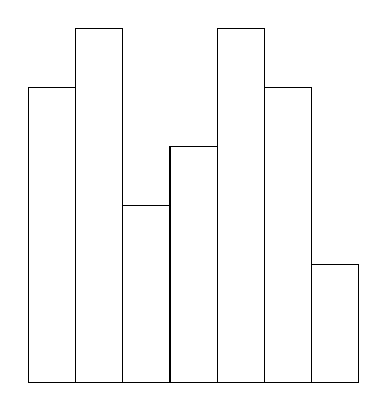
\begin{tikzpicture}[xscale=0.6, yscale=0.75]
            \draw (0,0) rectangle (1,5);
            \draw (1,0) rectangle (2,6);
            \draw (2,0) rectangle (3,3);
            \draw (3,0) rectangle (4,4);
            \draw (4,0) rectangle (5,6);
            \draw (5,0) rectangle (6,5);
            \draw (6,0) rectangle (7,2);
        \end{tikzpicture}
    \end{figure}

    \begin{solution}
        应用扫描线算法,事件点序列为木板高度升序。
        \[
            S(m,n) = \begin{cases}
                \max \begin{cases}
                    (n-m+1) \cdot \min_{m \le i \le n}{h_i}      \\
                    S(m,\mathrm{argmin}_{m \le i \le n}{h_i} -1) \\
                    S(\mathrm{argmin}_{m \le i \le n}{h_i} + 1, n)
                \end{cases} & m < n \\
                h_m                             & m = n \\
                0                               & m > n
            \end{cases}
        \]
        子问题互不重叠,不需要使用动态规划。

        \textbf{伪代码见算法\ref{alg:0427:1}}
    \end{solution}

    \begin{algorithm}[!ht]
        \caption{最大内接矩形}\label{alg:0427:1}
        \begin{algorithmic}[1]
            \Require{$H[1 \dots n]$($n$块木板的高度)}
            \Ensure{$MaxArea$(最大面积)}
            \State $I \gets \Call{SortedList}{H, \mathsf{key=}H[i], \mathsf{value}=i}$
            \Comment{存储的是板子在$H$中的索引,只有顺序查找,用链表}
            \State $MaxArea \gets -1$
            \State $Q \gets \Call{Queue}{\ }$
            \State $\Call{Queue.Push}{Q, (1,n)}$
            \While {$(x,y) \gets \Call{Queue.Pop}{Q}$}
            \If {$y > x$}
            \State $idx \gets \Call{List.findFirst}{I, [x,y]}$ \Comment{找到$[x,y]$区间内最低的板子$idx$}
            \State $area \gets H[idx] \cdot (y-x+1)$ \Comment{算面积}
            \State $MaxArea \gets area$ if $MaxArea < area$
            \State $\Call{Queue.Push}{Q,(x, idx-1)}$ \Comment{添加两个字问题}
            \State $\Call{Queue.Push}{Q,(idx+1, y)}$
            \State $\Call{List.Remove}{I, idx}$   \Comment{移除这块板子}
            \ElsIf {$y = x$}
            \State $area \gets H[x]$ \Comment{算面积}
            \State $MaxArea \gets area$ if $MaxArea < area$
            \State $\Call{List.Remove}{I, x}$   \Comment{移除这块板子}
            \EndIf
            \EndWhile
        \end{algorithmic}
    \end{algorithm}

    \question 平面有两组点,如何证明存在直线可以将这两组点分开?
    \begin{solution}
        \begin{enumerate}
            \item 对两组点分别求凸包,$O(\log n)$
            \item 判断两个凸包是否相交,$O(n)$
        \end{enumerate}
    \end{solution}
\end{questions}
